% !TEX TS-program = pdflatexmk
\documentclass[12pt]{article}

% Layout.
\usepackage[top=1in, bottom=0.75in, left=1in, right=1in, headheight=1in, headsep=6pt]{geometry}

% Fonts.
\usepackage{mathptmx}
\usepackage[scaled=0.86]{helvet}
\renewcommand{\emph}[1]{\textsf{\textbf{#1}}}
\newcommand{\ans}[1][1in]{\rule{#1}{.5pt}}

\usepackage[parfill]{parskip}

% Misc packages.
\usepackage{amsmath,amssymb,latexsym}
\usepackage{graphicx,hyperref}
\usepackage{array}
\usepackage{xcolor}
\usepackage{multicol,tikz}
\usepackage{tabularx,colortbl,booktabs,xparse}
\usepackage{enumitem}

\definecolor{roadcolor}{RGB}{100,120,180}
\definecolor{mstcolor}{RGB}{210,60,50}
\definecolor{nodecolor}{RGB}{30,80,160}
\definecolor{nodebg}{RGB}{220,235,255}
\definecolor{mstnode}{RGB}{255,240,220}

% Rotation: \rot[<angle>][<width>]{<stuff>}
\NewDocumentCommand{\rot}{O{45} O{1em} m}{\makebox[#2][l]{\rotatebox{#1}{#3}}}%

\usepackage{fancyhdr}
\pagestyle{fancy} 
\lhead{\large\sf\textbf{MATH F113X: Kruskal's Algorithm}}
%\chead{\large\sf\textbf{lecture notes}}
%\rhead{\large\sf\textbf{Day 1}}

\begin{document}

Goals:
\begin{itemize}
\item Understand the terms: tree, spanning tree, minimum cost spanning tree
\item Understand how to use Kruskal's Algorithm to find a minimum cost spanning tree
\item Know of applications of minimum cost spanning trees
\end{itemize}

%====================================================
% FIGURE 1: WEIGHTED ROAD GRAPH
%====================================================
\begin{center}
{\Large\bfseries Weighted Road Graph: 48 Contiguous U.S.\ State Capitals}\\[2pt]
{\small Edge weights = approximate road distance in miles. Each capital connected to its 4--5 nearest neighbors.}
\end{center}

\vspace{2pt}

\begin{center}
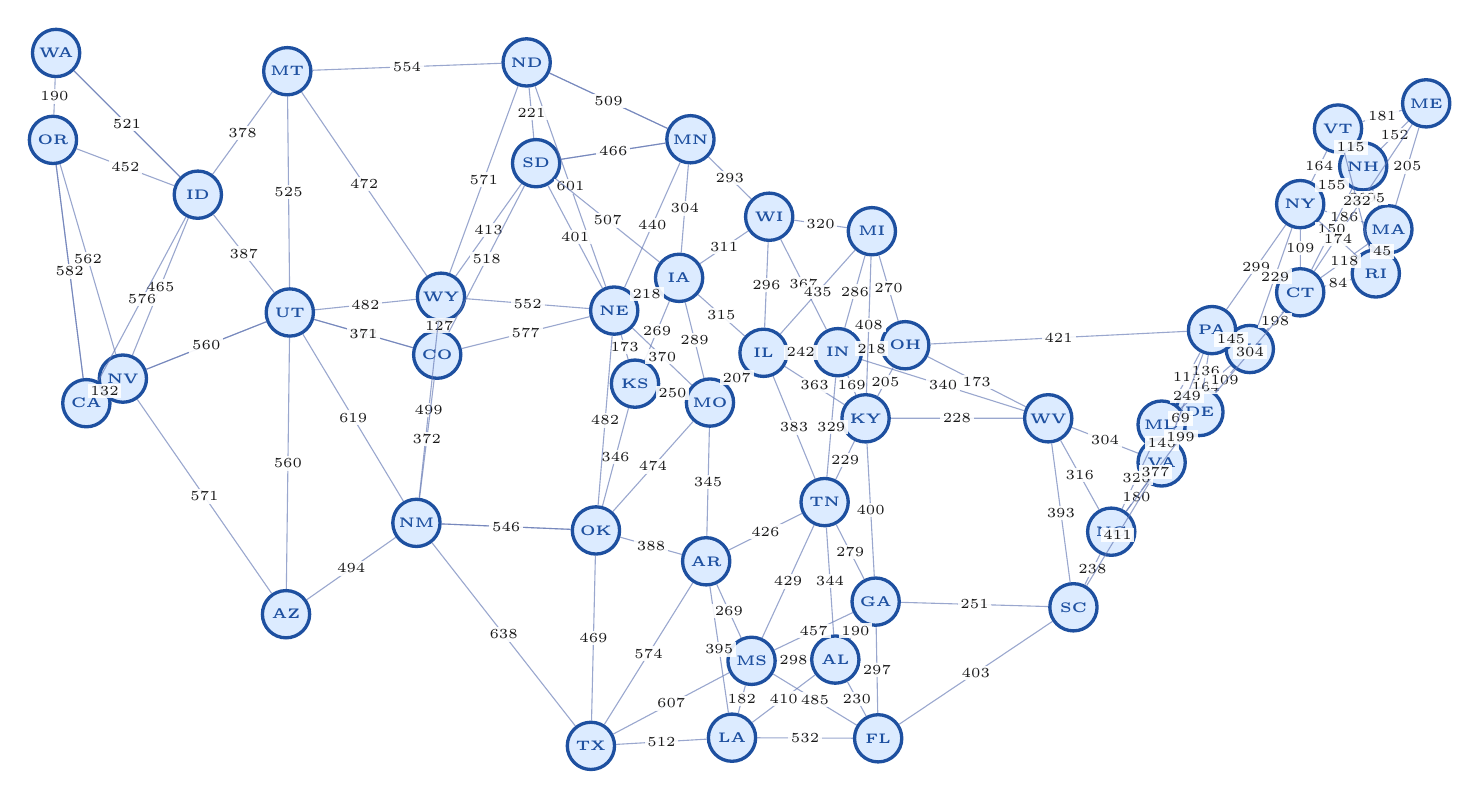
\begin{tikzpicture}[
  capital/.style={
    circle, draw=nodecolor, fill=nodebg, very thick,
    minimum size=6mm, inner sep=1pt, font=\bfseries\scriptsize, text=nodecolor
  },
  road/.style={draw=roadcolor, thin, opacity=0.65},
  weight/.style={fill=white, inner sep=1pt, font=\tiny, text=black, opacity=0.9, pos=0.5},
  scale=0.8
]

% ---- NODES ----
  \node[capital] (MontgomeryAL) at (12.42,1.37) {\tiny AL};
  \node[capital] (PhoenixAZ) at (3.70,2.09) {\tiny AZ};
  \node[capital] (LittleRockAR) at (10.37,2.93) {\tiny AR};
  \node[capital] (SacramentoCA) at (0.53,5.44) {\tiny CA};
  \node[capital] (DenverCO) at (6.10,6.21) {\tiny CO};
  \node[capital] (HartfordCT) at (19.80,7.20) {\tiny CT};
  \node[capital] (DoverDE) at (18.20,5.30) {\tiny DE};
  \node[capital] (TallahasseeFL) at (13.10,0.12) {\tiny FL};
  \node[capital] (AtlantaGA) at (13.06,2.29) {\tiny GA};
  \node[capital] (BoiseID) at (2.30,8.75) {\tiny ID};
  \node[capital] (SpringfieldIL) at (11.28,6.24) {\tiny IL};
  \node[capital] (IndianapolisIN) at (12.46,6.25) {\tiny IN};
  \node[capital] (DesMoinesIA) at (9.94,7.43) {\tiny IA};
  \node[capital] (TopekaKS) at (9.24,5.75) {\tiny KS};
  \node[capital] (FrankfortKY) at (12.90,5.20) {\tiny KY};
  \node[capital] (BatonRougeLA) at (10.78,0.13) {\tiny LA};
  \node[capital] (AugustaME) at (21.80,10.20) {\tiny ME};
  \node[capital] (AnnapolisMD) at (17.60,5.10) {\tiny MD};
  \node[capital] (BostonMA) at (21.20,8.20) {\tiny MA};
  \node[capital] (LansingMI) at (13.00,8.17) {\tiny MI};
  \node[capital] (StPaulMN) at (10.12,9.63) {\tiny MN};
  \node[capital] (JacksonMS) at (11.09,1.35) {\tiny MS};
  \node[capital] (JeffersonCityMO) at (10.43,5.45) {\tiny MO};
  \node[capital] (HelenaMT) at (3.72,10.71) {\tiny MT};
  \node[capital] (LincolnNE) at (8.91,6.91) {\tiny NE};
  \node[capital] (CarsonCityNV) at (1.11,5.83) {\tiny NV};
  \node[capital] (ConcordNH) at (20.80,9.20) {\tiny NH};
  \node[capital] (TrentonNJ) at (19.00,6.30) {\tiny NJ};
  \node[capital] (SantaFeNM) at (5.77,3.54) {\tiny NM};
  \node[capital] (AlbanyNY) at (19.80,8.60) {\tiny NY};
  \node[capital] (RaleighNC) at (16.80,3.40) {\tiny NC};
  \node[capital] (BismarckND) at (7.52,10.85) {\tiny ND};
  \node[capital] (ColumbusOH) at (13.53,6.36) {\tiny OH};
  \node[capital] (OklahomaCityOK) at (8.62,3.42) {\tiny OK};
  \node[capital] (SalemOR) at (0.00,9.62) {\tiny OR};
  \node[capital] (HarrisburgPA) at (18.40,6.60) {\tiny PA};
  \node[capital] (ProvidenceRI) at (21.00,7.50) {\tiny RI};
  \node[capital] (ColumbiaSC) at (16.20,2.20) {\tiny SC};
  \node[capital] (PierreSD) at (7.67,9.25) {\tiny SD};
  \node[capital] (NashvilleTN) at (12.25,3.87) {\tiny TN};
  \node[capital] (AustinTX) at (8.54,0.00) {\tiny TX};
  \node[capital] (SaltLakeCityUT) at (3.76,6.88) {\tiny UT};
  \node[capital] (MontpelierVT) at (20.40,9.80) {\tiny VT};
  \node[capital] (RichmondVA) at (17.60,4.50) {\tiny VA};
  \node[capital] (OlympiaWA) at (0.05,11.00) {\tiny WA};
  \node[capital] (CharlestonWV) at (15.80,5.20) {\tiny WV};
  \node[capital] (MadisonWI) at (11.37,8.40) {\tiny WI};
  \node[capital] (CheyenneWY) at (6.16,7.13) {\tiny WY};

% ---- ROAD EDGES ----
  \draw[road] (AlbanyNY) -- node[weight] {\tiny 186} (BostonMA);
  \draw[road] (AlbanyNY) -- node[weight] {\tiny 155} (ConcordNH);
  \draw[road] (AlbanyNY) -- node[weight] {\tiny 299} (HarrisburgPA);
  \draw[road] (AlbanyNY) -- node[weight] {\tiny 109} (HartfordCT);
  \draw[road] (AlbanyNY) -- node[weight] {\tiny 164} (MontpelierVT);
  \draw[road] (AnnapolisMD) -- node[weight] {\tiny 69} (DoverDE);
  \draw[road] (AnnapolisMD) -- node[weight] {\tiny 119} (HarrisburgPA);
  \draw[road] (AnnapolisMD) -- node[weight] {\tiny 326} (RaleighNC);
  \draw[road] (AnnapolisMD) -- node[weight] {\tiny 146} (RichmondVA);
  \draw[road] (AnnapolisMD) -- node[weight] {\tiny 164} (TrentonNJ);
  \draw[road] (AtlantaGA) -- node[weight] {\tiny 251} (ColumbiaSC);
  \draw[road] (AtlantaGA) -- node[weight] {\tiny 190} (MontgomeryAL);
  \draw[road] (AtlantaGA) -- node[weight] {\tiny 279} (NashvilleTN);
  \draw[road] (AtlantaGA) -- node[weight] {\tiny 297} (TallahasseeFL);
  \draw[road] (AtlantaGA) -- node[weight] {\tiny 457} (JacksonMS);
  \draw[road] (AugustaME) -- node[weight] {\tiny 205} (BostonMA);
  \draw[road] (AugustaME) -- node[weight] {\tiny 152} (ConcordNH);
  \draw[road] (AugustaME) -- node[weight] {\tiny 299} (HartfordCT);
  \draw[road] (AugustaME) -- node[weight] {\tiny 181} (MontpelierVT);
  \draw[road] (AustinTX) -- node[weight] {\tiny 512} (BatonRougeLA);
  \draw[road] (AustinTX) -- node[weight] {\tiny 574} (LittleRockAR);
  \draw[road] (AustinTX) -- node[weight] {\tiny 469} (OklahomaCityOK);
  \draw[road] (BatonRougeLA) -- node[weight] {\tiny 182} (JacksonMS);
  \draw[road] (BatonRougeLA) -- node[weight] {\tiny 395} (LittleRockAR);
  \draw[road] (BatonRougeLA) -- node[weight] {\tiny 410} (MontgomeryAL);
  \draw[road] (BismarckND) -- node[weight] {\tiny 571} (CheyenneWY);
  \draw[road] (BismarckND) -- node[weight] {\tiny 601} (LincolnNE);
  \draw[road] (BismarckND) -- node[weight] {\tiny 221} (PierreSD);
  \draw[road] (BismarckND) -- node[weight] {\tiny 509} (StPaulMN);
  \draw[road] (BoiseID) -- node[weight] {\tiny 465} (CarsonCityNV);
  \draw[road] (BoiseID) -- node[weight] {\tiny 378} (HelenaMT);
  \draw[road] (BoiseID) -- node[weight] {\tiny 521} (OlympiaWA);
  \draw[road] (BoiseID) -- node[weight] {\tiny 452} (SalemOR);
  \draw[road] (BoiseID) -- node[weight] {\tiny 387} (SaltLakeCityUT);
  \draw[road] (BostonMA) -- node[weight] {\tiny 95} (ConcordNH);
  \draw[road] (BostonMA) -- node[weight] {\tiny 118} (HartfordCT);
  \draw[road] (BostonMA) -- node[weight] {\tiny 45} (ProvidenceRI);
  \draw[road] (CarsonCityNV) -- node[weight] {\tiny 132} (SacramentoCA);
  \draw[road] (CarsonCityNV) -- node[weight] {\tiny 560} (SaltLakeCityUT);
  \draw[road] (CharlestonWV) -- node[weight] {\tiny 173} (ColumbusOH);
  \draw[road] (CharlestonWV) -- node[weight] {\tiny 228} (FrankfortKY);
  \draw[road] (CharlestonWV) -- node[weight] {\tiny 316} (RaleighNC);
  \draw[road] (CharlestonWV) -- node[weight] {\tiny 304} (RichmondVA);
  \draw[road] (CheyenneWY) -- node[weight] {\tiny 127} (DenverCO);
  \draw[road] (CheyenneWY) -- node[weight] {\tiny 413} (PierreSD);
  \draw[road] (CheyenneWY) -- node[weight] {\tiny 482} (SaltLakeCityUT);
  \draw[road] (CheyenneWY) -- node[weight] {\tiny 499} (SantaFeNM);
  \draw[road] (ColumbiaSC) -- node[weight] {\tiny 238} (RaleighNC);
  \draw[road] (ColumbusOH) -- node[weight] {\tiny 205} (FrankfortKY);
  \draw[road] (ColumbusOH) -- node[weight] {\tiny 218} (IndianapolisIN);
  \draw[road] (ColumbusOH) -- node[weight] {\tiny 270} (LansingMI);
  \draw[road] (ConcordNH) -- node[weight] {\tiny 150} (HartfordCT);
  \draw[road] (ConcordNH) -- node[weight] {\tiny 115} (MontpelierVT);
  \draw[road] (DenverCO) -- node[weight] {\tiny 518} (PierreSD);
  \draw[road] (DenverCO) -- node[weight] {\tiny 482} (SaltLakeCityUT);
  \draw[road] (DenverCO) -- node[weight] {\tiny 372} (SantaFeNM);
  \draw[road] (DesMoinesIA) -- node[weight] {\tiny 289} (JeffersonCityMO);
  \draw[road] (DesMoinesIA) -- node[weight] {\tiny 218} (LincolnNE);
  \draw[road] (DesMoinesIA) -- node[weight] {\tiny 311} (MadisonWI);
  \draw[road] (DesMoinesIA) -- node[weight] {\tiny 315} (SpringfieldIL);
  \draw[road] (DesMoinesIA) -- node[weight] {\tiny 304} (StPaulMN);
  \draw[road] (DesMoinesIA) -- node[weight] {\tiny 269} (TopekaKS);
  \draw[road] (DoverDE) -- node[weight] {\tiny 136} (HarrisburgPA);
  \draw[road] (DoverDE) -- node[weight] {\tiny 109} (TrentonNJ);
  \draw[road] (FrankfortKY) -- node[weight] {\tiny 169} (IndianapolisIN);
  \draw[road] (FrankfortKY) -- node[weight] {\tiny 229} (NashvilleTN);
  \draw[road] (HarrisburgPA) -- node[weight] {\tiny 249} (RichmondVA);
  \draw[road] (HarrisburgPA) -- node[weight] {\tiny 145} (TrentonNJ);
  \draw[road] (HartfordCT) -- node[weight] {\tiny 84} (ProvidenceRI);
  \draw[road] (HartfordCT) -- node[weight] {\tiny 198} (TrentonNJ);
  \draw[road] (HelenaMT) -- node[weight] {\tiny 525} (SaltLakeCityUT);
  \draw[road] (IndianapolisIN) -- node[weight] {\tiny 286} (LansingMI);
  \draw[road] (IndianapolisIN) -- node[weight] {\tiny 329} (NashvilleTN);
  \draw[road] (IndianapolisIN) -- node[weight] {\tiny 242} (SpringfieldIL);
  \draw[road] (JacksonMS) -- node[weight] {\tiny 269} (LittleRockAR);
  \draw[road] (JacksonMS) -- node[weight] {\tiny 298} (MontgomeryAL);
  \draw[road] (JeffersonCityMO) -- node[weight] {\tiny 345} (LittleRockAR);
  \draw[road] (JeffersonCityMO) -- node[weight] {\tiny 207} (SpringfieldIL);
  \draw[road] (JeffersonCityMO) -- node[weight] {\tiny 250} (TopekaKS);
  \draw[road] (LansingMI) -- node[weight] {\tiny 320} (MadisonWI);
  \draw[road] (LincolnNE) -- node[weight] {\tiny 401} (PierreSD);
  \draw[road] (LincolnNE) -- node[weight] {\tiny 173} (TopekaKS);
  \draw[road] (LittleRockAR) -- node[weight] {\tiny 388} (OklahomaCityOK);
  \draw[road] (MadisonWI) -- node[weight] {\tiny 296} (SpringfieldIL);
  \draw[road] (MadisonWI) -- node[weight] {\tiny 293} (StPaulMN);
  \draw[road] (MontgomeryAL) -- node[weight] {\tiny 344} (NashvilleTN);
  \draw[road] (MontgomeryAL) -- node[weight] {\tiny 230} (TallahasseeFL);
  \draw[road] (MontpelierVT) -- node[weight] {\tiny 232} (ProvidenceRI);
  \draw[road] (OklahomaCityOK) -- node[weight] {\tiny 346} (TopekaKS);
  \draw[road] (OlympiaWA) -- node[weight] {\tiny 190} (SalemOR);
  \draw[road] (PhoenixAZ) -- node[weight] {\tiny 494} (SantaFeNM);
  \draw[road] (PierreSD) -- node[weight] {\tiny 466} (StPaulMN);
  \draw[road] (RaleighNC) -- node[weight] {\tiny 180} (RichmondVA);
  \draw[road] (SacramentoCA) -- node[weight] {\tiny 582} (SalemOR);
  \draw[road] (SaltLakeCityUT) -- node[weight] {\tiny 619} (SantaFeNM);
  \draw[road] (AlbanyNY) -- node[weight] {\tiny 174} (ProvidenceRI);
  \draw[road] (AtlantaGA) -- node[weight] {\tiny 400} (FrankfortKY);
  \draw[road] (AustinTX) -- node[weight] {\tiny 607} (JacksonMS);
  \draw[road] (BatonRougeLA) -- node[weight] {\tiny 532} (TallahasseeFL);
  \draw[road] (BoiseID) -- node[weight] {\tiny 576} (SacramentoCA);
  \draw[road] (CarsonCityNV) -- node[weight] {\tiny 562} (SalemOR);
  \draw[road] (CharlestonWV) -- node[weight] {\tiny 393} (ColumbiaSC);
  \draw[road] (CharlestonWV) -- node[weight] {\tiny 340} (IndianapolisIN);
  \draw[road] (ColumbiaSC) -- node[weight] {\tiny 411} (RichmondVA);
  \draw[road] (ColumbiaSC) -- node[weight] {\tiny 403} (TallahasseeFL);
  \draw[road] (ColumbusOH) -- node[weight] {\tiny 421} (HarrisburgPA);
  \draw[road] (DenverCO) -- node[weight] {\tiny 577} (LincolnNE);
  \draw[road] (DesMoinesIA) -- node[weight] {\tiny 507} (PierreSD);
  \draw[road] (DoverDE) -- node[weight] {\tiny 304} (HartfordCT);
  \draw[road] (DoverDE) -- node[weight] {\tiny 377} (RaleighNC);
  \draw[road] (DoverDE) -- node[weight] {\tiny 199} (RichmondVA);
  \draw[road] (FrankfortKY) -- node[weight] {\tiny 363} (SpringfieldIL);
  \draw[road] (IndianapolisIN) -- node[weight] {\tiny 367} (MadisonWI);
  \draw[road] (JacksonMS) -- node[weight] {\tiny 429} (NashvilleTN);
  \draw[road] (JacksonMS) -- node[weight] {\tiny 485} (TallahasseeFL);
  \draw[road] (JeffersonCityMO) -- node[weight] {\tiny 370} (LincolnNE);
  \draw[road] (JeffersonCityMO) -- node[weight] {\tiny 474} (OklahomaCityOK);
  \draw[road] (LansingMI) -- node[weight] {\tiny 435} (SpringfieldIL);
  \draw[road] (LincolnNE) -- node[weight] {\tiny 440} (StPaulMN);
  \draw[road] (LincolnNE) -- node[weight] {\tiny 482} (OklahomaCityOK);
  \draw[road] (LittleRockAR) -- node[weight] {\tiny 426} (NashvilleTN);
  \draw[road] (NashvilleTN) -- node[weight] {\tiny 383} (SpringfieldIL);
  \draw[road] (OklahomaCityOK) -- node[weight] {\tiny 616} (SantaFeNM);
  \draw[road] (AlbanyNY) -- node[weight] {\tiny 229} (TrentonNJ);
  \draw[road] (BismarckND) -- node[weight] {\tiny 509} (StPaulMN);
  \draw[road] (FrankfortKY) -- node[weight] {\tiny 408} (LansingMI);

% ---- EXTRA WESTERN EDGES ----
  % Phoenix connections
  \draw[road] (PhoenixAZ) -- node[weight] {\tiny 571} (CarsonCityNV);
  \draw[road] (PhoenixAZ) -- node[weight] {\tiny 560} (SaltLakeCityUT);
  % Helena connections
  \draw[road] (HelenaMT) -- node[weight] {\tiny 554} (BismarckND);
  \draw[road] (HelenaMT) -- node[weight] {\tiny 472} (CheyenneWY);
  % Oregon / Washington to California
  \draw[road] (SalemOR) -- node[weight] {\tiny 582} (SacramentoCA);
  \draw[road] (OlympiaWA) -- node[weight] {\tiny 521} (BoiseID);
  % Nevada–Utah–Colorado triangle
  \draw[road] (CarsonCityNV) -- node[weight] {\tiny 560} (SaltLakeCityUT);
  \draw[road] (SaltLakeCityUT) -- node[weight] {\tiny 371} (DenverCO);
  % New Mexico–Oklahoma link
  \draw[road] (SantaFeNM) -- node[weight] {\tiny 546} (OklahomaCityOK);
  % Texas–New Mexico
  \draw[road] (AustinTX) -- node[weight] {\tiny 638} (SantaFeNM);
  % Wyoming–South Dakota–Nebraska loop
  \draw[road] (CheyenneWY) -- node[weight] {\tiny 552} (LincolnNE);
  \draw[road] (PierreSD) -- node[weight] {\tiny 466} (StPaulMN);

\end{tikzpicture}
\end{center}

\newpage
%====================================================
% FIGURE 2: MINIMUM SPANNING TREE
%====================================================
\begin{center}
{\Large\bfseries Minimum Weight Spanning Tree (Kruskal's Algorithm)}\\[2pt]
{\small Total MST weight $\approx \mathbf{11{,}411}$ miles. Red edges form the unique spanning tree of minimum total road distance.}
\end{center}

\vspace{2pt}

\begin{center}
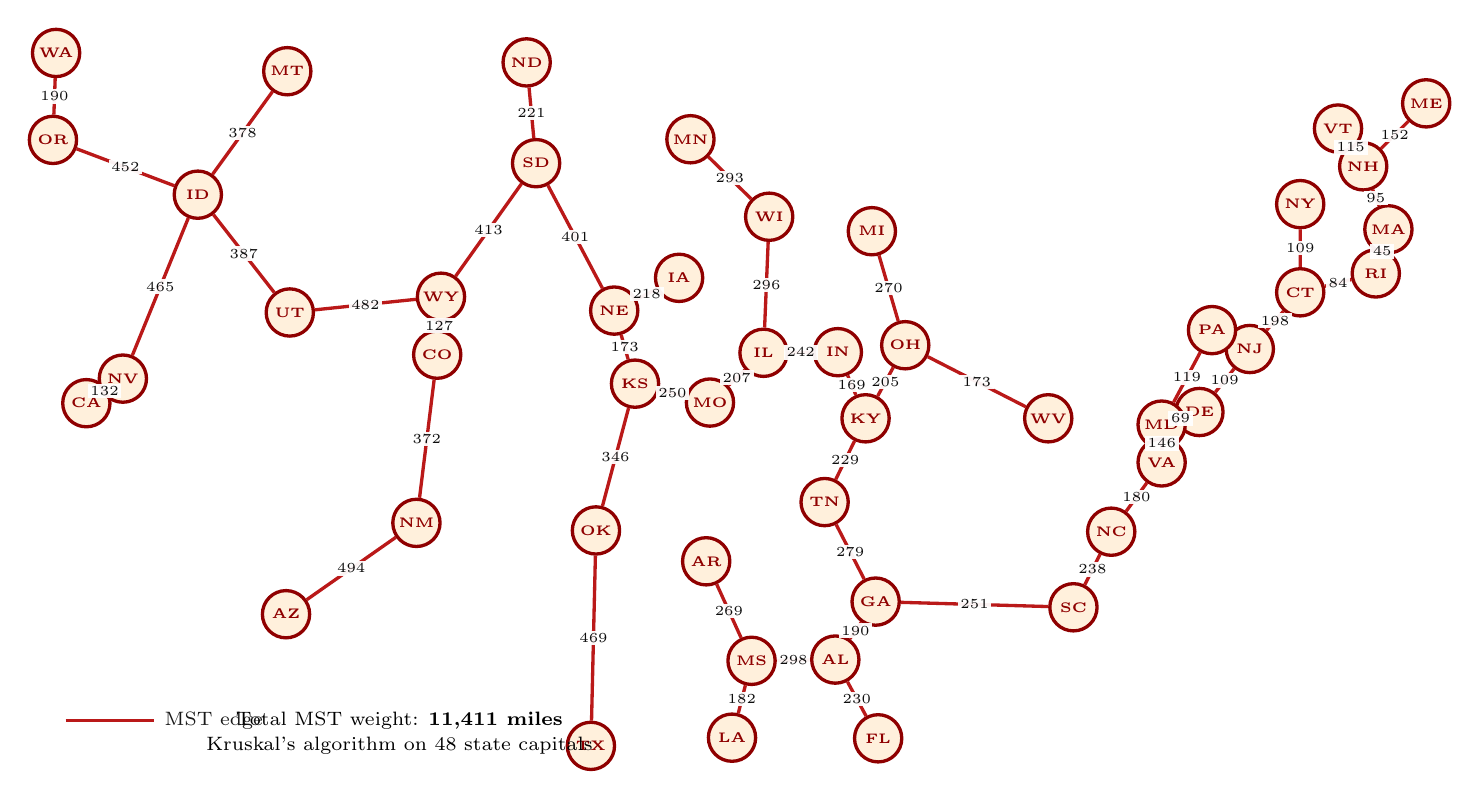
\begin{tikzpicture}[
  capital/.style={
    circle, draw=mstcolor!80!black, fill=mstnode, very thick,
    minimum size=6mm, inner sep=1pt, font=\bfseries\scriptsize, text=mstcolor!80!black
  },
  mstedge/.style={draw=mstcolor, very thick, opacity=0.9},
  weight/.style={fill=white, inner sep=1pt, font=\tiny, text=black, opacity=0.95, pos=0.5},
  mstcolor/.style={RGB}{210,60,50},
  scale=0.8
]

\colorlet{mstcolor}{red!70!black}

% ---- NODES ----
  \node[capital] (MontgomeryAL) at (12.42,1.37) {\tiny AL};
  \node[capital] (PhoenixAZ) at (3.70,2.09) {\tiny AZ};
  \node[capital] (LittleRockAR) at (10.37,2.93) {\tiny AR};
  \node[capital] (SacramentoCA) at (0.53,5.44) {\tiny CA};
  \node[capital] (DenverCO) at (6.10,6.21) {\tiny CO};
  \node[capital] (HartfordCT) at (19.80,7.20) {\tiny CT};
  \node[capital] (DoverDE) at (18.20,5.30) {\tiny DE};
  \node[capital] (TallahasseeFL) at (13.10,0.12) {\tiny FL};
  \node[capital] (AtlantaGA) at (13.06,2.29) {\tiny GA};
  \node[capital] (BoiseID) at (2.30,8.75) {\tiny ID};
  \node[capital] (SpringfieldIL) at (11.28,6.24) {\tiny IL};
  \node[capital] (IndianapolisIN) at (12.46,6.25) {\tiny IN};
  \node[capital] (DesMoinesIA) at (9.94,7.43) {\tiny IA};
  \node[capital] (TopekaKS) at (9.24,5.75) {\tiny KS};
  \node[capital] (FrankfortKY) at (12.90,5.20) {\tiny KY};
  \node[capital] (BatonRougeLA) at (10.78,0.13) {\tiny LA};
  \node[capital] (AugustaME) at (21.80,10.20) {\tiny ME};
  \node[capital] (AnnapolisMD) at (17.60,5.10) {\tiny MD};
  \node[capital] (BostonMA) at (21.20,8.20) {\tiny MA};
  \node[capital] (LansingMI) at (13.00,8.17) {\tiny MI};
  \node[capital] (StPaulMN) at (10.12,9.63) {\tiny MN};
  \node[capital] (JacksonMS) at (11.09,1.35) {\tiny MS};
  \node[capital] (JeffersonCityMO) at (10.43,5.45) {\tiny MO};
  \node[capital] (HelenaMT) at (3.72,10.71) {\tiny MT};
  \node[capital] (LincolnNE) at (8.91,6.91) {\tiny NE};
  \node[capital] (CarsonCityNV) at (1.11,5.83) {\tiny NV};
  \node[capital] (ConcordNH) at (20.80,9.20) {\tiny NH};
  \node[capital] (TrentonNJ) at (19.00,6.30) {\tiny NJ};
  \node[capital] (SantaFeNM) at (5.77,3.54) {\tiny NM};
  \node[capital] (AlbanyNY) at (19.80,8.60) {\tiny NY};
  \node[capital] (RaleighNC) at (16.80,3.40) {\tiny NC};
  \node[capital] (BismarckND) at (7.52,10.85) {\tiny ND};
  \node[capital] (ColumbusOH) at (13.53,6.36) {\tiny OH};
  \node[capital] (OklahomaCityOK) at (8.62,3.42) {\tiny OK};
  \node[capital] (SalemOR) at (0.00,9.62) {\tiny OR};
  \node[capital] (HarrisburgPA) at (18.40,6.60) {\tiny PA};
  \node[capital] (ProvidenceRI) at (21.00,7.50) {\tiny RI};
  \node[capital] (ColumbiaSC) at (16.20,2.20) {\tiny SC};
  \node[capital] (PierreSD) at (7.67,9.25) {\tiny SD};
  \node[capital] (NashvilleTN) at (12.25,3.87) {\tiny TN};
  \node[capital] (AustinTX) at (8.54,0.00) {\tiny TX};
  \node[capital] (SaltLakeCityUT) at (3.76,6.88) {\tiny UT};
  \node[capital] (MontpelierVT) at (20.40,9.80) {\tiny VT};
  \node[capital] (RichmondVA) at (17.60,4.50) {\tiny VA};
  \node[capital] (OlympiaWA) at (0.05,11.00) {\tiny WA};
  \node[capital] (CharlestonWV) at (15.80,5.20) {\tiny WV};
  \node[capital] (MadisonWI) at (11.37,8.40) {\tiny WI};
  \node[capital] (CheyenneWY) at (6.16,7.13) {\tiny WY};

% ---- MST EDGES (47 edges, Kruskal's algorithm) ----
  \draw[mstedge] (BostonMA) -- node[weight] {\tiny 45} (ProvidenceRI);
  \draw[mstedge] (DoverDE) -- node[weight] {\tiny 69} (AnnapolisMD);
  \draw[mstedge] (HartfordCT) -- node[weight] {\tiny 84} (ProvidenceRI);
  \draw[mstedge] (BostonMA) -- node[weight] {\tiny 95} (ConcordNH);
  \draw[mstedge] (HartfordCT) -- node[weight] {\tiny 109} (AlbanyNY);
  \draw[mstedge] (DoverDE) -- node[weight] {\tiny 109} (TrentonNJ);
  \draw[mstedge] (ConcordNH) -- node[weight] {\tiny 115} (MontpelierVT);
  \draw[mstedge] (AnnapolisMD) -- node[weight] {\tiny 119} (HarrisburgPA);
  \draw[mstedge] (DenverCO) -- node[weight] {\tiny 127} (CheyenneWY);
  \draw[mstedge] (SacramentoCA) -- node[weight] {\tiny 132} (CarsonCityNV);
  \draw[mstedge] (AnnapolisMD) -- node[weight] {\tiny 146} (RichmondVA);
  \draw[mstedge] (AugustaME) -- node[weight] {\tiny 152} (ConcordNH);
  \draw[mstedge] (IndianapolisIN) -- node[weight] {\tiny 169} (FrankfortKY);
  \draw[mstedge] (TopekaKS) -- node[weight] {\tiny 173} (LincolnNE);
  \draw[mstedge] (ColumbusOH) -- node[weight] {\tiny 173} (CharlestonWV);
  \draw[mstedge] (RaleighNC) -- node[weight] {\tiny 180} (RichmondVA);
  \draw[mstedge] (BatonRougeLA) -- node[weight] {\tiny 182} (JacksonMS);
  \draw[mstedge] (MontgomeryAL) -- node[weight] {\tiny 190} (AtlantaGA);
  \draw[mstedge] (SalemOR) -- node[weight] {\tiny 190} (OlympiaWA);
  \draw[mstedge] (HartfordCT) -- node[weight] {\tiny 198} (TrentonNJ);
  \draw[mstedge] (FrankfortKY) -- node[weight] {\tiny 205} (ColumbusOH);
  \draw[mstedge] (SpringfieldIL) -- node[weight] {\tiny 207} (JeffersonCityMO);
  \draw[mstedge] (DesMoinesIA) -- node[weight] {\tiny 218} (LincolnNE);
  \draw[mstedge] (BismarckND) -- node[weight] {\tiny 221} (PierreSD);
  \draw[mstedge] (FrankfortKY) -- node[weight] {\tiny 229} (NashvilleTN);
  \draw[mstedge] (MontgomeryAL) -- node[weight] {\tiny 230} (TallahasseeFL);
  \draw[mstedge] (RaleighNC) -- node[weight] {\tiny 238} (ColumbiaSC);
  \draw[mstedge] (SpringfieldIL) -- node[weight] {\tiny 242} (IndianapolisIN);
  \draw[mstedge] (TopekaKS) -- node[weight] {\tiny 250} (JeffersonCityMO);
  \draw[mstedge] (AtlantaGA) -- node[weight] {\tiny 251} (ColumbiaSC);
  \draw[mstedge] (LittleRockAR) -- node[weight] {\tiny 269} (JacksonMS);
  \draw[mstedge] (LansingMI) -- node[weight] {\tiny 270} (ColumbusOH);
  \draw[mstedge] (AtlantaGA) -- node[weight] {\tiny 279} (NashvilleTN);
  \draw[mstedge] (StPaulMN) -- node[weight] {\tiny 293} (MadisonWI);
  \draw[mstedge] (SpringfieldIL) -- node[weight] {\tiny 296} (MadisonWI);
  \draw[mstedge] (MontgomeryAL) -- node[weight] {\tiny 298} (JacksonMS);
  \draw[mstedge] (TopekaKS) -- node[weight] {\tiny 346} (OklahomaCityOK);
  \draw[mstedge] (DenverCO) -- node[weight] {\tiny 372} (SantaFeNM);
  \draw[mstedge] (BoiseID) -- node[weight] {\tiny 378} (HelenaMT);
  \draw[mstedge] (BoiseID) -- node[weight] {\tiny 387} (SaltLakeCityUT);
  \draw[mstedge] (LincolnNE) -- node[weight] {\tiny 401} (PierreSD);
  \draw[mstedge] (PierreSD) -- node[weight] {\tiny 413} (CheyenneWY);
  \draw[mstedge] (BoiseID) -- node[weight] {\tiny 452} (SalemOR);
  \draw[mstedge] (BoiseID) -- node[weight] {\tiny 465} (CarsonCityNV);
  \draw[mstedge] (OklahomaCityOK) -- node[weight] {\tiny 469} (AustinTX);
  \draw[mstedge] (SaltLakeCityUT) -- node[weight] {\tiny 482} (CheyenneWY);
  \draw[mstedge] (PhoenixAZ) -- node[weight] {\tiny 494} (SantaFeNM);

% ---- Legend ----
\draw[mstedge] (0.2,0.4) -- (1.6,0.4) node[right,font=\scriptsize,text=black] {MST edge};
\node[font=\scriptsize,text=black] at (5.5,0.4) {Total MST weight: \textbf{11,411 miles}};
\node[font=\scriptsize,text=black] at (5.5,0.0) {Kruskal's algorithm on 48 state capitals};

\end{tikzpicture}
\end{center}



\newpage
\begin{enumerate}
\item Definitions
	\begin{enumerate}
	\item \emph{weighted graph}
	\vfill
	\item \textbf{tree}
	\vfill
	\item \textbf{spanning tree}
	\vfill
	\item \textbf{minimum cost spanning tree}
	\vfill
	\end{enumerate}
\item Example: \\
%\fbox{
\begin{minipage}{.5\linewidth}
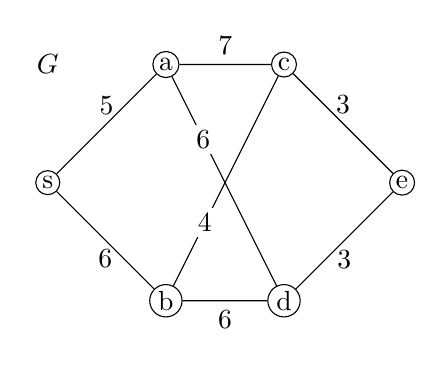
\begin{tikzpicture}[scale=1.5]
\node at (0,1){$G$};
\node[draw,circle, inner sep=1pt](s) at (0,0){s};
\node[draw,circle, inner sep=1pt](a) at (1,1){a};
\node[draw,circle, inner sep=1pt](b) at (1,-1){b};
\node[draw,circle, inner sep=1pt](c) at (2,1){c};
\node[draw,circle, inner sep=1pt](d) at (2,-1){d};
\node[draw,circle, inner sep=1pt](e) at (3,0){e};
\draw (s) -- (a) node [midway,above]{5};
\draw (s) -- (b) node [midway,below]{6};
\draw (a) -- (c) node [midway,above]{7};
\draw (a) -- (d) node [pos = .3, inner sep = 2pt, fill = white]{6};
\draw (b) -- (c) node [pos = .3, inner sep = 2pt, fill = white]{4};
\draw (b) -- (d) node [midway,below]{6};
\draw (d) -- (e) node [midway,below]{3};
\draw (c) -- (e) node [midway,above]{3};
\end{tikzpicture}
\end{minipage}
%}

\newpage
\item
\fbox{Kruskal's Algorithm}

\textbf{input:} a graph, $G$, with costs (or weights) on the edges\\
\textbf{output:} a spanning tree, $T$, of minimum cost\\
\textbf{Steps:}
\begin{enumerate}
	\item (Initialization Step:) $T$ is a graph on the vertex set of $G$ but with no edges.
	\item (Iterative Step:) 
		\begin{enumerate}
		\item Select the cheapest unused edge in the graph. (Ties are broken alphabetically.)
		\item If the edge does \emph{not} create a cycle, add the edge to $T$. Otherwise, reject the edge.
		\item Mark the edge as used.
		\item If $T$ is a spanning tree, STOP. Otherwise return to the beginning of the iterative step.
		\end{enumerate}
\end{enumerate}

\item Use Kruskal's Algorithm to find the minimum cost spanning tree for the graph $G$ below.

\vspace{1cm}
%%G%%
\fbox{
\begin{minipage}{.5\linewidth}
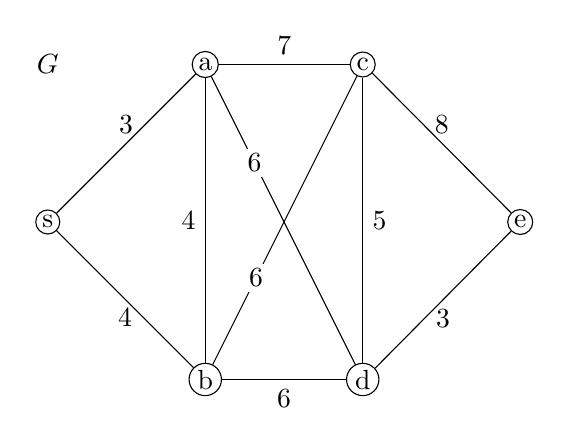
\begin{tikzpicture}[scale=2]
\node at (0,1){$G$};
\node[draw,circle, inner sep=1pt](s) at (0,0){s};
\node[draw,circle, inner sep=1pt](a) at (1,1){a};
\node[draw,circle, inner sep=1pt](b) at (1,-1){b};
\node[draw,circle, inner sep=1pt](c) at (2,1){c};
\node[draw,circle, inner sep=1pt](d) at (2,-1){d};
\node[draw,circle, inner sep=1pt](e) at (3,0){e};
\draw (s) -- (a) node [midway,above]{3};
\draw (s) -- (b) node [midway,below]{4};
\draw (a) -- (b) node [midway,left]{4};
\draw (a) -- (c) node [midway,above]{7};
\draw (a) -- (d) node [pos = .3, inner sep = 2pt, fill = white]{6};
\draw (b) -- (c) node [pos = .3, inner sep = 2pt, fill = white]{6};
\draw (b) -- (d) node [midway,below]{6};
\draw (d) -- (e) node [midway,below]{3};
\draw (c) -- (e) node [midway,above]{8};
\draw (c) -- (d) node [midway,right]{5};
\end{tikzpicture}
\end{minipage}
}
%%%%%%%
%%T%%
\fbox{
\begin{minipage}{.5\linewidth}
\begin{tikzpicture}[scale=2]
\node at (1,1.2){$\quad$};
\node at (1,-1.2){$\quad$};
\node at (0,1){$T$};
\node[draw,circle, inner sep=1pt](s) at (0,0){s};
\node[draw,circle, inner sep=1pt](a) at (1,1){a};
\node[draw,circle, inner sep=1pt](b) at (1,-1){b};
\node[draw,circle, inner sep=1pt](c) at (2,1){c};
\node[draw,circle, inner sep=1pt](d) at (2,-1){d};
\node[draw,circle, inner sep=1pt](e) at (3,0){e};
\end{tikzpicture}
\end{minipage}
}
%%%%%%%
\vfill
\begin{minipage}[t]{.5\linewidth}
\begin{tabular}{ c | p{2in} | p{2in}}
Used? &edges & weights\\ \hline
& \\
& \\
& \\& \\& \\& \\& \\& \\& \\% \\& \\& \\
 \end{tabular}
 \end{minipage}
 
 
\vfill
\item Think of an application of Kruskal's Algorithm.

\vfill
\end{enumerate}
\end{document}